%! alt Regular hexagon ABCDEF with centre O. The dashed triangle ACE joins alternate vertices and covers half of the hexagon. The highlighted triangle PQR joins the midpoints P, Q and R of sides AB, CD and EF, and has the same centre O, with OP shorter than OA.
%! after_paragraph 2
%! scale 1
% The shared preamble of every Cevian figure. pipeline/figures turns these colours into theme-aware paint,
% and refuses any other colour, so draw only with them:
%   figink (lines and labels), figaux (construction lines), figaccent (the object the argument turns on),
%   figtint and figaccenttint (light fills).
\documentclass[border=1.5pt]{standalone}
\usepackage{tkz-euclide}
\definecolor{figink}{RGB}{0,0,0}
\definecolor{figaux}{RGB}{85,85,85}
\definecolor{figaccent}{RGB}{192,57,43}
\definecolor{figtint}{RGB}{221,221,221}
\definecolor{figaccenttint}{RGB}{245,213,208}
% tkz-euclide's defaults draw circles, compasses and marks in 50% grey and fill points with a tint.
\makeatletter
\def\tkz@otherlinecolor{figink}
\def\tkz@euc@circlecolor{figink}
\def\tkz@euc@compasscolor{figink}
\def\tkz@euc@mkcolor{figink}
\def\tkz@mk@fill{figink}
\def\tkz@euc@pointfillcolor{figink}
\makeatother
\tkzSetUpLine[color=figink,line width=.7pt]
\tkzSetUpArc[color=figink,line width=.7pt]
\tkzSetUpCompass[color=figink,line width=.5pt]
\tkzSetUpPoint[color=figink,fill=figink,size=3.1pt]
\tikzset{
  every picture/.style={line cap=round,line join=round,color=figink},
  circle style/.append style={color=figink,line width=.7pt},
  aux/.style={color=figaux,line width=.45pt,dash pattern=on 2.6pt off 2pt},
  key/.style={color=figaccent,line width=1pt},
  mk/.style={color=figink,line width=.5pt},
  lbl/.style={color=figink,inner sep=2.2pt},
  len/.style={color=figink,inner sep=1.5pt,font=\small},
}

\begin{document}
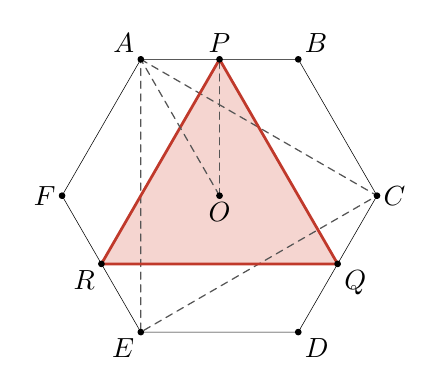
\begin{tikzpicture}
\tkzDefPoint(0.0,0.0){O} %! O = (0, 0)
\tkzDefPoint(-1.0000000,1.7320508){A} %! A = polar(O, 2, 120)
\tkzDefPoint(1.0000000,1.7320508){B} %! B = polar(O, 2, 60)
\tkzDefPoint(2.0000000,0.0){C} %! C = polar(O, 2, 0)
\tkzDefPoint(1.0000000,-1.7320508){D} %! D = polar(O, 2, -60)
\tkzDefPoint(-1.0000000,-1.7320508){E} %! E = polar(O, 2, -120)
\tkzDefPoint(-2.0000000,0.0000000000000000000000000000000000000000000000000086696674){F} %! F = polar(O, 2, 180)
\tkzDefPoint(0.0000000000000000000000000000000000000000000000000013363824,1.7320508){P} %! P = mid(A, B)
\tkzDefPoint(1.5000000,-0.86602540){Q} %! Q = mid(C, D)
\tkzDefPoint(-1.5000000,-0.86602540){R} %! R = mid(E, F)
%! fact area(A, C, E) / area(A, B, C, D, E, F) == 1/2
%! fact area(P, Q, R) / area(A, B, C, D, E, F) == 3/8
%! fact (dist(O, P) / dist(O, A))**2 == 3/4
%! fact angle(P, O, Q) == 120
\tkzFillPolygon[color=figaccenttint](P,Q,R)
\tkzDrawPolygon(A,B,C,D,E,F)
\tkzDrawPolygon[aux](A,C,E)
\tkzDrawPolygon[key](P,Q,R)
\tkzDrawSegments[aux](O,A O,P)
\tkzDrawPoints(A,B,C,D,E,F,O,P,Q,R)
\tkzLabelPoint[above left,lbl](A){$A$}
\tkzLabelPoint[above right,lbl](B){$B$}
\tkzLabelPoint[right,lbl](C){$C$}
\tkzLabelPoint[below right,lbl](D){$D$}
\tkzLabelPoint[below left,lbl](E){$E$}
\tkzLabelPoint[left,lbl](F){$F$}
\tkzLabelPoint[above,lbl](P){$P$}
\tkzLabelPoint[below right,lbl](Q){$Q$}
\tkzLabelPoint[below left,lbl](R){$R$}
\tkzLabelPoint[below,lbl](O){$O$}
\end{tikzpicture}
\end{document}
